\documentclass[titlepage]{jarticle}
\usepackage[dvipdfmx]{graphicx}
\usepackage{here}
\begin{document}
 \begin{titlepage}
  \begin{center}
   \vspace*{100truept}
   {\Large 令和三年度体育祭計画書}\\
   \vspace{10truept}
   \begin{eqnarray*}
    期日&&10月12日(火)\\
    雨天延期日&&10月19日(火)\\
   \end{eqnarray*}
   \\
   \vspace{250truept}
   {\large 総責任者}\\
   \vspace{10truept}
   体育委員長\\
   \vspace{10truept}
   電子制御工学科 三年\\
   \vspace{10truept}
   本間 三暉\\
   \vspace{10truept}
   (ec31121m@nagaoka-ct.ac.jp)
  \end{center}
 \end{titlepage}
 \part*{}
 \section{日時}
  10月12日(火) 8:40~14:40
 \section{プログラム}
  \begin{eqnarray*}
   08:40~08:50&&グラウンド集合・点呼\\
   08:50~09:30&&開会式\\
   09:40~10:20&&学科対抗宅配競争\\
   10:30~11:15&&借人競争\\
   11:25~12:00&&学科対抗玉入れ\\
   12:00~12:50&&昼休み\\
   13:00~13:40&&部活対抗パン掴み競走\\
   13:50~14:10&&学科対抗リレー\\
   14:20~14:40&&閉会式
  \end{eqnarray*}
 \section{今年度の目標}
   \begin{itemize}
    \item 充分に水分補給する。\\
    \item 怪我や病気に気をつける。\\
   \end{itemize}
 \section{開会式・閉会式}
  開閉会式の並び方を図\ref{open_close}に示す。
  \subsection{開会式}
  \begin{center}
  \begin{tabbing}
   \hspace{8zh}\=\hspace{10zh}\kill
    開会宣言\\
    校歌静聴\>2分\\
    体育委員長挨拶\>1分\\
    校長挨拶\>3分\\
    団長挨拶\>各1分×5学科=5分\\
    学校体操\>4分\\

    競技上の注意\>1分\\
    諸連絡想定\>3分
  \end{tabbing}
  \end{center}
  \subsection{閉会式}
  \begin{center}
  \begin{tabbing}
   \hspace{8zh}\=\hspace{10zh}\kill
    結果発表、表彰\>3分\\
    団長挨拶\>各1分×5学科=5分\\
    体育委員長挨拶\>1分\\
    学生主事挨拶\>3分\\
    閉会宣言\\
    諸連絡想定\>3分\\
    クラス写真撮影\>自由参加
  \end{tabbing}
  \end{center}
  \begin{figure}[h]
   \centering
   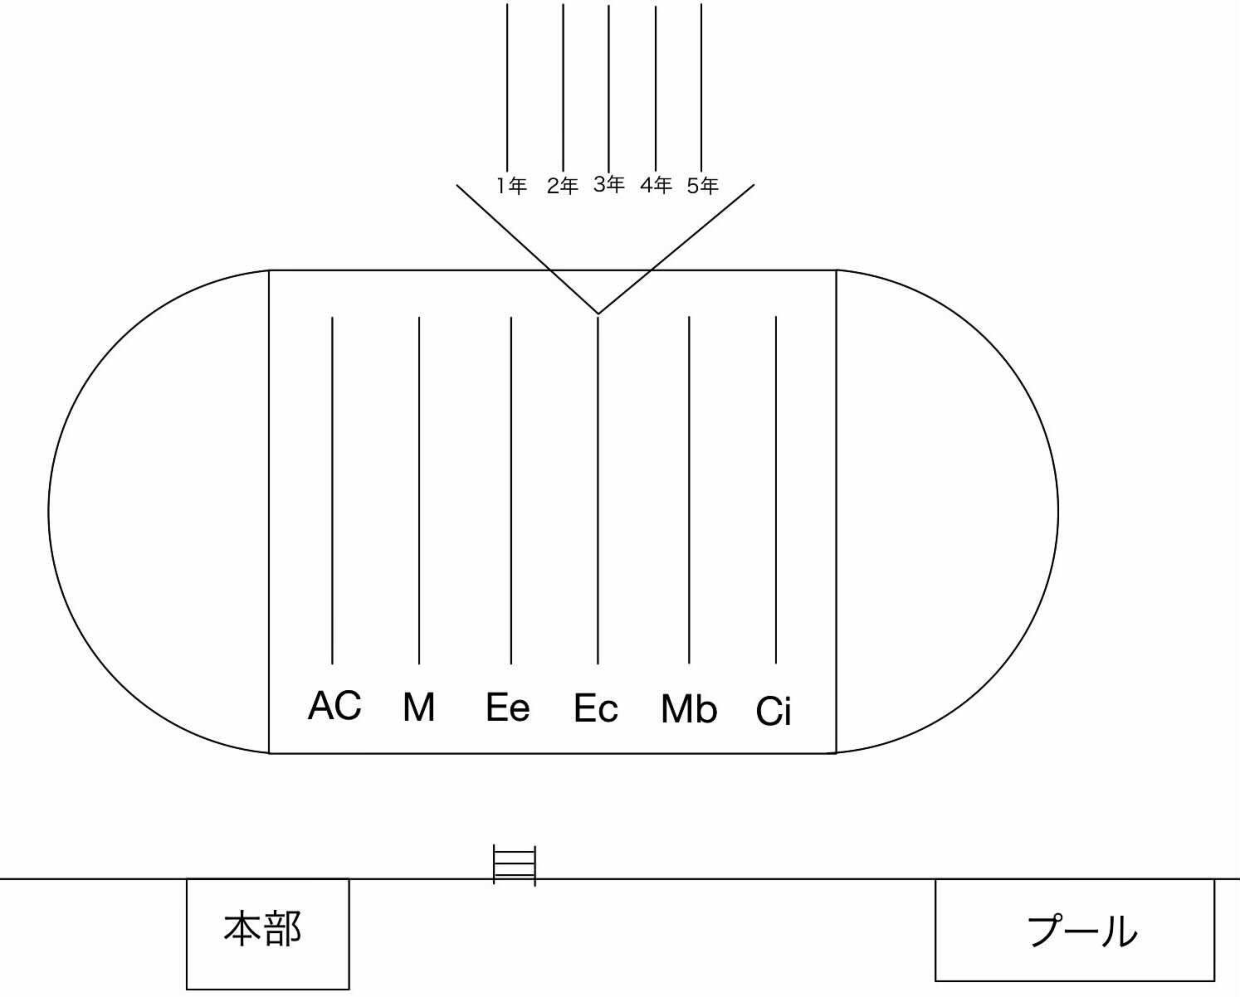
\includegraphics[width=12cm]{open_close.pdf}
   \caption{開閉会式並び方}
   \label{open_close}
  \end{figure}
  \section{競技種目}
   以下競技種目について記述していく。
 \clearpage
 \setcounter{section}{0}
 \begin{center}
  \part*{全体競技}
 \end{center}
 \section{全体競技ルール}
  \subsection{一年生について}
   \begin{itemize}
    \item 一年生は学科ごとではなく、クラスごとに競技に参加し以下のように学科に所属するものとする。
    \begin{eqnarray*}
     一組&&物質工学科\\
     二組&&環境都市工学科\\
     三組&&機械工学科\\
     四組&&電気電子システム工学科\\
     五組&&電子制御工学科\\
    \end{eqnarray*}
    \item 一年生が入賞した場合、所属する学科に点数が入る。
   \end{itemize}
  \subsection{競技上の注意点}
   \begin{itemize} 
    \item 集合時間は各試合の7~10分前とする。各競技説明に集合時間が明記してある場合はそちらを優先する。
   \item 一人が同じ競技に二度参加することはできない。例えば、リレーで二人分走る、複数の部活に所属しているのでパン掴み競争で一回戦目と二回戦目に出る。などということはしてはならない。
  \item 競技開始時点で人が集まらなかった場合には競技に参加することはできない。
    \item 競技中の途中参加は認めない。
    \item 他学科からの助っ人は認めない。 
    \item 審判の指示には必ず従うこと。
    \item 暴力、運営の妨害、他人を傷つけるような言動を行った場合、それらの行為を行った学生は、競技中であれば失格とし、また、競技中であるないにかかわらず所属している学科の点数から減点を行う。 
    \item RBは教員のチームとする。
   \end{itemize}
  \subsection{服装について}
   \begin{itemize}
    \item 運動しやすい服装で競技を行うこと。
    \item 装飾品を外して競技に参加すること。(例:腕時計、ピアス、ネックレス、スマホ等)
    \item グラウンド内でスパイクを履いてはいけない。 
    \item 競技中に着用するビブスと帽子、バトンは学科ごとに決められた色のものを着用する。それぞれの色は表\ref{colour}に示す。
   \end{itemize}
   \begin{table}[H]
    \caption{ビブスの色}
    \centering
    \label{colour}
    \begin{tabular}{c||ccccc}
       &M &Ee &Ec &Mb &Ci \\ \hline\hline
     ビブス&青&黄&オレンジ&黒&緑\\
     バトン&青&黄&赤&ピンク&緑\\
    \end{tabular}
   \end{table}
  \subsection{コロナ対策に関する注意点}
   \begin{itemize}
    \item 競技前後に手洗いうがい消毒を徹底すること。四号館外の水道を使うのが好ましい。
    \item 競技以外では{\large 必ず}マスクを着用すること。
    \item 競技のときはマスクを外してもよいが、向かい合ってしゃべるのはなるべく控えること。
    \item 競技の際にマスクの有無に関わらず、大声を出すのは控えること。減点や失格とする場合がある。
    \item リレーや玉入れなどの共有物品を使う競技では特に手の消毒をすること。
   \end{itemize}
  \subsection{その他の注意点}
   \begin{itemize}
    \item グラウンド内では、飲み物は自由に飲んでいいが食事をしてはいけない。
    \item 体調が悪くなった場合は無理せず保健室へ。
    \item けがをした場合は本部に連絡すること。
    \item 疑問点がある場合は本部へ行くか近くの役員へ相談すること。
   \end{itemize}
 \section{待機場所、及び集合場所について}
  \begin{itemize}
   \item 今年は新型コロナウイルス蔓延防止の観点から待機場所、観戦席を設けない。
   \item 校舎側のグラウンド管理室前を待機場所とする。
   \begin{figure}[H]
    \centering
    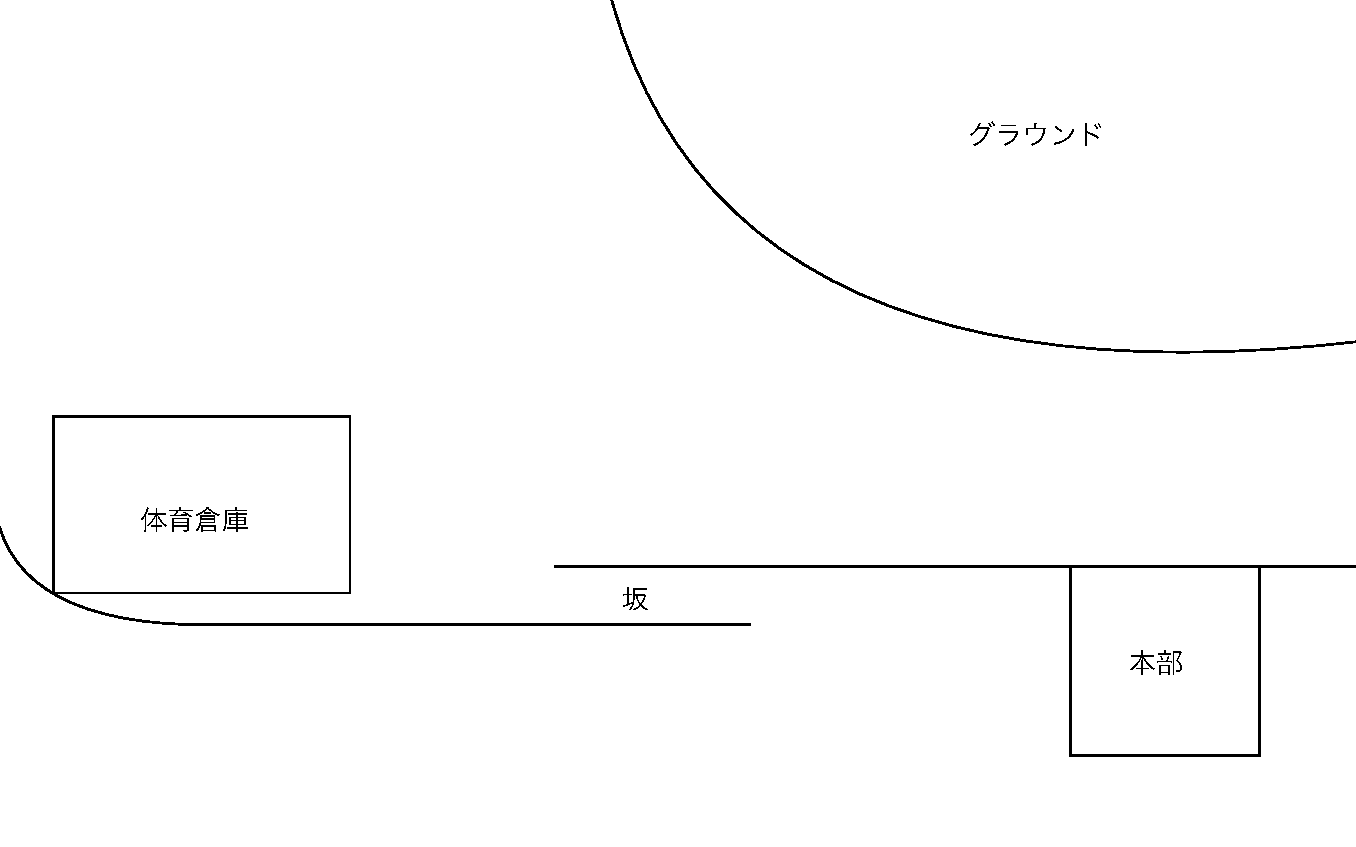
\includegraphics[width=12cm]{syugo.pdf}
    \caption{集合場所}
   \end{figure}
%
  \end{itemize}
\clearpage
 \setcounter{section}{0}
%ここから競技説明
%1宅配競争
 \section{学科対抗宅配競争}
  \subsection{競技内容}
   \subsubsection{競技ルール}
    \begin{itemize}
     \item 荷物(段ボール箱)を持った状態で50m先の次の走者のところまで走っていき、アンカー以外はその走者の荷物(段ボール箱)の上に重ねる。また、アンカーが荷物を運んだ時点でゴールとする。
     \item 荷物を落としてしまった場合、もう一度荷物を積み上げ、落とした地点からもう一度スタートすることとする。また、積み上げるのは荷物を落とした人のみが行うこととする。
     \item 受け渡し時に落とした場合はこれから運ぶ人が積み上げることとする。
     \item 積み上げるときに荷物に触っていいのは一人だけである。複数人で積み上げようとした場合には失格となる場合がある。
     \item 5学科同時に行い、全部で2試合行う。
    \end{itemize}
   \subsubsection{専攻科について}
    \begin{itemize}
     \item 専攻科生は参加不可
    \end{itemize}
   \subsubsection{競技人数}
    \begin{itemize}
    \item 1クラス4人、各学科合計20人、計100名。これを2レースに分ける。
    \end{itemize}
   \subsubsection{点数配分}
    \begin{itemize}
     \item 1位から90点、70点、50点、40点、30点とする。
     \item 同点の場合は同じ順位(タイ)とし同じ点数を与える。
    \end{itemize}
  \subsection{競技図}
   \begin{figure}[H]
    \centering
    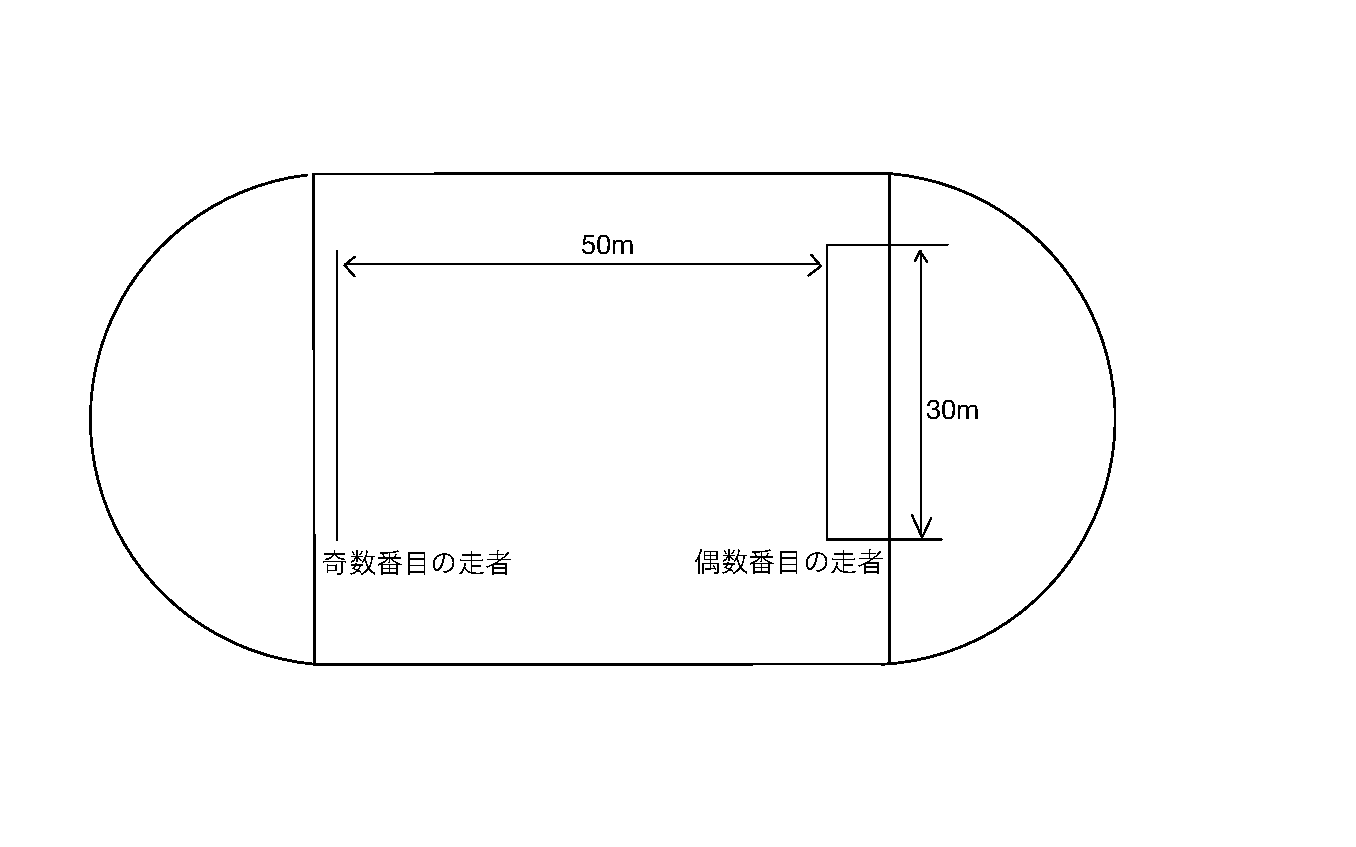
\includegraphics[width=12cm]{box2.pdf}
    \caption{宅配競技図}
   \end{figure}
  \subsection{対戦表}
   \begin{table}[H]
    \centering
    \begin{tabular}{ccc}
       &集合時間&試合時間 \\ \hline\hline
     一回戦(各クラス2人)&9:30&9:40~9:50\\
     二回戦(各クラス2人)&9:50&10:00~10:10\\
    \end{tabular}
   \end{table}
  \subsection{使用器具}
   \begin{table}[H]
    \begin{tabular}{cccc}
     物品名&数量&管理者 &備考\\ \hline\hline
     カラーコーン&4個&体育委員会&高さ60cm\\
     ダンボール&50箱分&学生会&300×300×150\\
    \end{tabular}
   \end{table}
  \subsection{審判}
   学生会役員5人で行う。
   \begin{itemize}
    \item 荷物補給、走者誘導4人、順位記録1人。
   \end{itemize}
  \subsection{その他の注意点}
   \begin{itemize}
    \item 特になし。
   \end{itemize}
\clearpage
%2
 \section{借り人競争}
  \subsection{競技内容}
   \subsubsection{競技ルール}
    \begin{itemize}
     \item 学年単位で行う。1クラス必ず4人参加。本部左手のコーンとコーンの間からスタートする。制限時間は3分とする。
     \item スタートの合図で一斉にお題の書かれた紙と拡声器を取りに行く。
     \item グラウンドから外れてお題の人を探しに行く。
     \item 対象の人物を見つけたらグラウンドに入りお題を行う。ただし、グラウンド人工芝生外でのお題実行はやり直しとする。
     \item お題をクリアしたら本部右手のゴールへまっすぐ向かう。ただし、反対側からのゴールは認められない。基本的には全チームがゴールするまで行う。
     \item 計6試合行う。
     \item 探すときは大声を出してはいけない。その代わりに拡声器を使う事ができる。
    \end{itemize}
   \subsubsection{専攻科について}
    \begin{itemize}
     \item 専攻科の参加は可能。RB、学生会も同様。
    \end{itemize}
   \subsubsection{競技人数}
    \begin{itemize}
     \item 各クラス4名選出する。 
     \item 走順は以下に示す。 
     \begin{enumerate}
      \item 1年生 
      \item 2年生 
      \item 3年生 
      \item 4年生 
      \item 5年生 
      \item 専攻科、RB、学生会
     \end{enumerate}
    \end{itemize}
   \subsubsection{点数配分}
    \begin{itemize}
     \item 1位の学科のチームから順に130点、80点、60点、50点、40点とする。
    \end{itemize}
  \subsection{競技図}
   \begin{figure}[H]
    \centering
    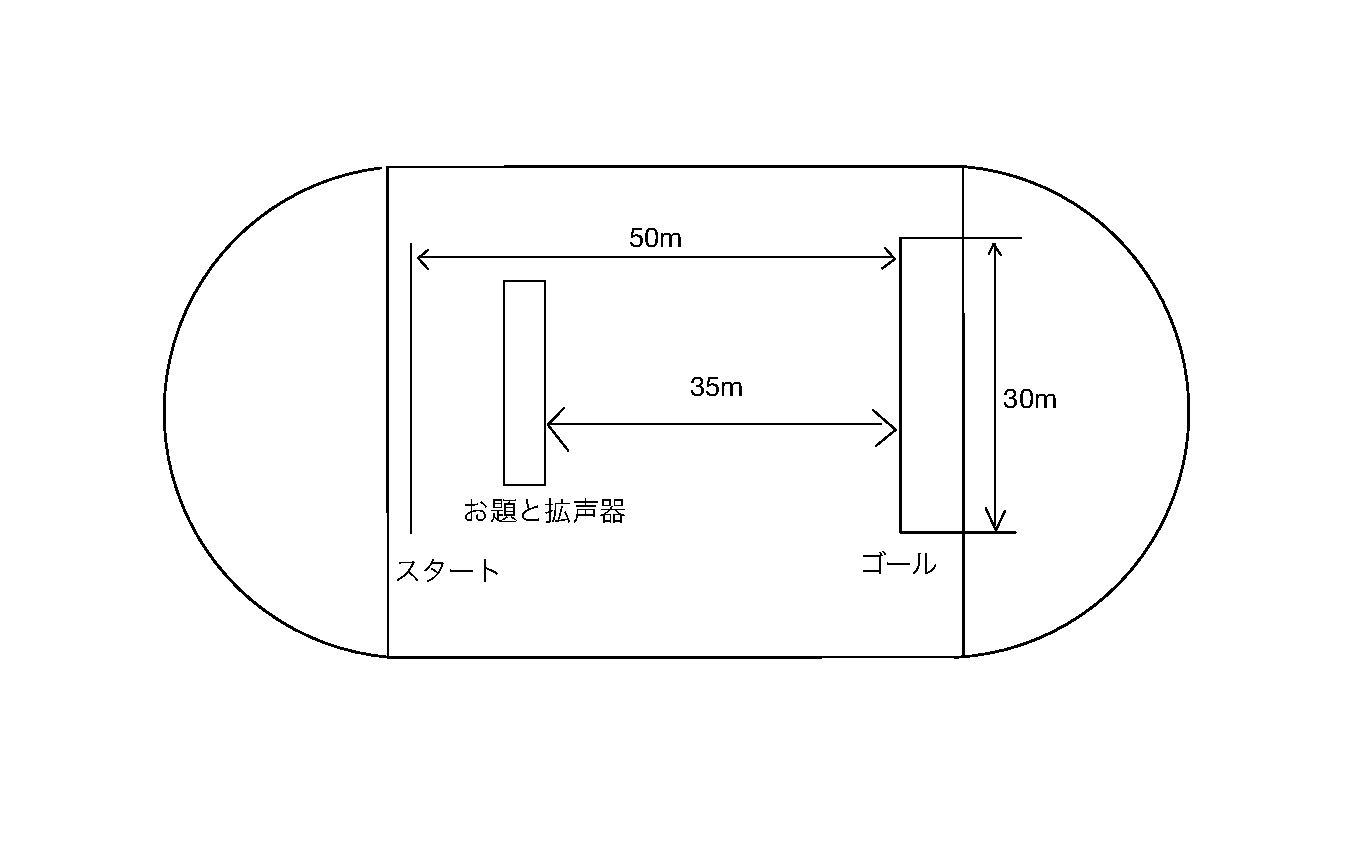
\includegraphics[width=12cm]{borrow.pdf}
    \caption{借り人競技図}
   \end{figure}
  \subsection{使用器具}
   \begin{table}[H]
    \begin{tabular}{cccc}
     物品名&数量&管理者 &備考\\ \hline\hline
A4白紙&120枚&学生会&\\
コーン&4本&学生会体育委員&\\
マイク&1本&学生課&\\
拡声器&あるだけ&学生課&借りれる分だけ借りる\\
賞品&6個&学生会体育委員会&\\
    \end{tabular}
   \end{table}
  \subsection{審判}
   \begin{itemize}
   \item お題の紙を置いている周辺に学生会から審判を4人役員2人配置する。 
   \item MC1人と教員1名を配置する。
   \end{itemize} 
  \subsection{その他注意点}
   \begin{itemize}
   \item 殴る、蹴る、相手を引っ張る・抑えるなどの妨害行為は禁止とする。 
   \end{itemize}
  \clearpage
%3
 \section{学科対抗玉入れ}
  \subsection{競技内容}
   \subsubsection{競技ルール}
    \begin{itemize}
     \item かごの中に玉を投げて入れる。
     \item 1試合1分とする。
     \item かごの周りに直径 4m , 6m , 7m の円を設ける。
     \item 紅白玉はそれぞれ90個使用する。
     \item 3mの円の中に玉を30個、4mの円から6mの円の中に60個まんべんなく配置する。
     \item 1,2年生は3mの円の中で、3~5年生は4mの円から6mの円の中で行い、試合中はその範囲から出てはならない。
     \item 競技に参加する人はスタートの合図があるまで7mの円の中には入ってはいけない。
     \item 複数人で騎馬や土台に類するものを構成してはならない。
     \item 6mの円の外に行ってしまった玉を取ることはできない。
     \item かごの中に入った玉の数を集計し玉の数が多かった順に順位をつける。
     \item 試合は2学科ずつ同時に行う。
     \item かごの高さは4m44cmとする。
     \item 終了のピストルが鳴ってから投げ入れられたものは無効とする。
     \item 玉を数える際は学生会役員のみ拡声器を使い声を出すこととする。
    \end{itemize}
   \subsubsection{専攻科について}
    \begin{itemize}
     \item 専攻科生はRBと合同チームで参加可能。
    \end{itemize}
   \subsubsection{競技人数}
    \begin{itemize}
     \item1クラス5人、各学科合計25人、計150名。
     \item RBと専攻科チームは25人とする。
    \end{itemize}
   \subsubsection{点数配分}
    \begin{itemize}
     \item 1位から順に100点、80点、60点、50点、40点とする。
     \item 同点の場合は同じ順位(タイ)とし同じ点数を与える。
    \end{itemize}
  \subsection{競技図}
   \begin{figure}[H]
    \centering
    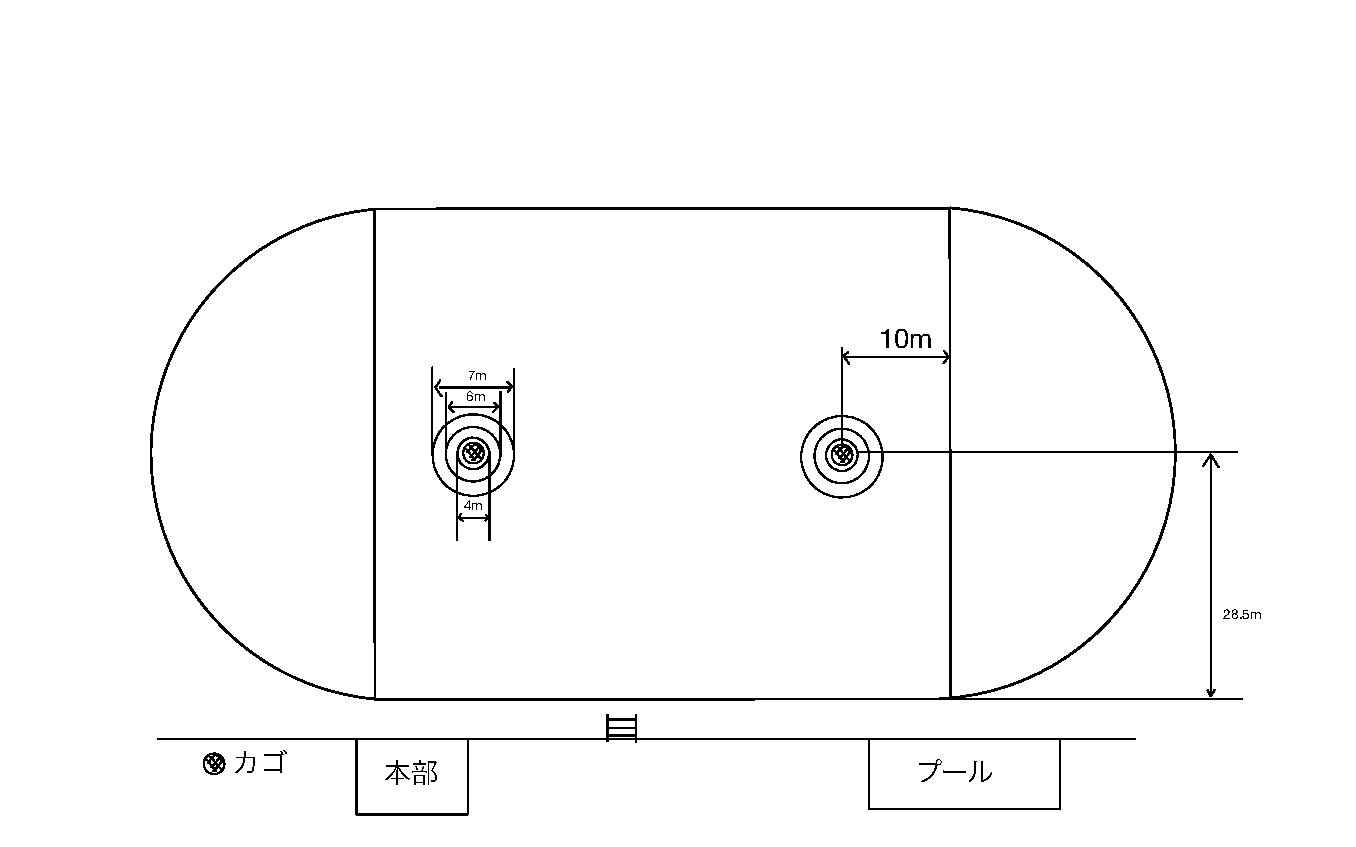
\includegraphics[width=12cm]{ballin2.pdf}
    \caption{玉入れ競技図}
   \end{figure}
  \subsection{対戦表}
   \begin{table}[H]
    \begin{tabular}{ccccc}
     &集合時間&競技時間&プール側(白)&六号館側(紅)\\ \hline\hline
     一回戦&11:15&11:25~11:30&Ci&Ee\\
     二回戦&11:30&11:40~11:45&Mb&M\\
     三回戦&11:45&11:50~12:00&Ec&RB\&Ac\\
    \end{tabular}
   \end{table}
  \subsection{使用器具}
   \begin{table}[H]
    \begin{tabular}{cccc}
     物品名&数量&管理者 &備考\\ \hline\hline
紅玉&99個&学生会体育委員会&予備9個\\
白玉&96個&学生会体育委員&予備6個\\
かご(紅白)&2個&学生会体育委員会&最大4m44cm\\
    \end{tabular}
   \end{table}
  \subsection{審判}
    学生会役員6人で行う。
   \begin{itemize}

    \item 棒を支える\&玉を数える人4人
    \item 線から出ないか確認するための人2人
    \item 役員は安全のため頭に何かを被る(帽子やタオルなど)
   \end{itemize}
  \subsection{その他の注意点}
   \begin{itemize}
    \item 選手、審判ともにマスクを付け試合が終わったら互いに離れること。
   \end{itemize}
\clearpage
%4pan
 \section{部活対抗パン掴み競争}
  \subsection{競技内容}
   \subsubsection{競技ルール}
    \begin{itemize}
     \item ここで言う部活は同好会を含む。
     \item 学生便覧266ページを元に作成する。
     \item 1試合最大10組の部活が走り、計5試合行う。
     \item どのようにかしてパンをゴールまで運ばなければならない。パンがゴールラインを過ぎた時点でゴールとする。
     \item 競技中にパンを口に含む行為を禁止する。
     \item パンをとる際、パンに直接手で触れることを禁止とする。但し、部活に関係する物の使用は認める。
     \item 各試合で1位がゴールしたらピストルを鳴らす。(競技はまだ続ける)
     \item すべての部活がゴールし、試合終了したらピストルを鳴らす。
     \item 1試合最大3分とする。時間を超えた場合は強制終了する。
     \item 1~4試合目で1着ゴールした部活で決勝戦を行う。
     \item パンを破壊する行為は失格とする。
     \item 
    \end{itemize}
   \subsubsection{専攻科について}
    \begin{itemize}
     \item 専攻科生は各部活1人まで参加できる。(専攻科生のみでの参加は不可。)
    \end{itemize}
   \subsubsection{競技人数}
    \begin{itemize}
     \item 1部活最大3人まで参加可能(専攻科生込み)
     \item 全部活合計0~114人(抽選会で参加部活、レース順を決定)
    \end{itemize}
   \subsubsection{点数配分}
     どの学科にも点数は入らないが、下記の部活に賞品として部費を授与する。
競技のパフォーマンスの順位付けについてはteamsのリアクション機能を使い、決定する。
    \begin{itemize}
     \item パフォーマンスはteamsのリアクション機能を使用し、順位を決める。
     \item 決勝戦上位2部活(計2部活)
     \item パフォーマンス賞(計3部活)
    \end{itemize}
   \subsubsection{危険行為}
    \begin{itemize}
     \item 部活に関係する物を使用する際、周りに気を付けること。振り回したり、投げたりしてはならない。
     \item 部活としてのアイテムの持ち込みはよいが、危険物・グラウンドを汚すものを持ち込んではならない。
    \end{itemize}
  \subsection{競技図}
   \begin{figure}[H]
    \centering
    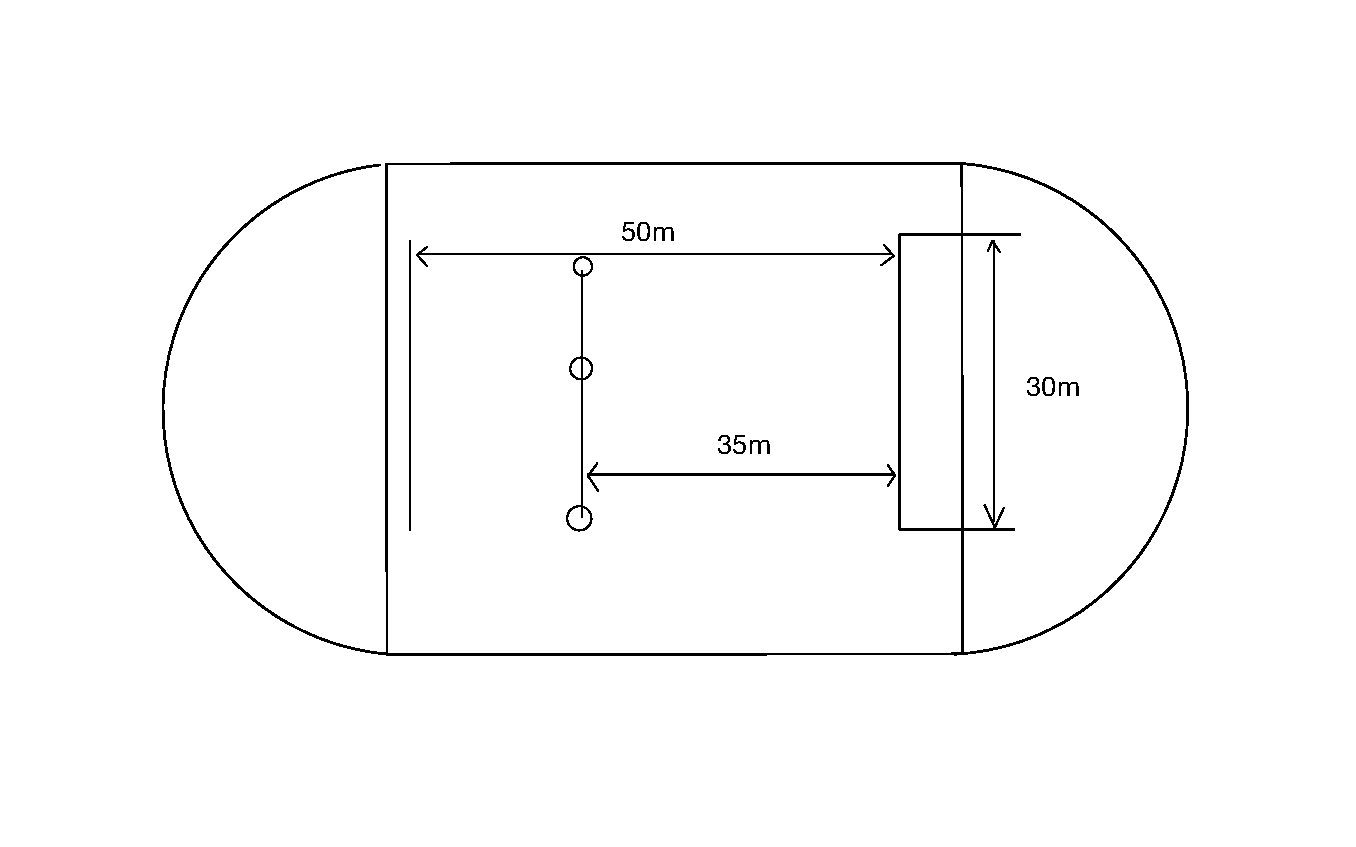
\includegraphics[width=12cm]{bread.pdf}
    \caption{パン掴み競技図}
   \end{figure}
  \subsection{対戦表}
   \subsubsection{参加部活}
    \textgt{第1試合} テニス部、卓球部、サッカー部、柔道部、バドミントン部、ハンドボール部、水泳部、ダンス部\\

    \textgt{第2試合} 陸上競技部、山岳部、バスケットボール部バレーボール部、ソフトテニス部、剣道部、スキー部、硬式野球部、ゴルフ部\\

    \textgt{第3試合} 吹奏楽部、インターアクトクラブ、軽音楽部、ロボティクス部、デザイン部、制御システム研究同好会、模型同好会\\

    \textgt{第4試合} 美術部、写真部、電算機部、文芸部、英語部、化学部、書道部アントレプレナー部\\

    \textgt{第5試合} 各試合1位の部活
   \subsubsection{競技時間}
    \begin{table}[H]
     \begin{tabular}{c|cccc}
       &集合時間&競技時間\\ \hline\hline
      第1試合&13:00&13:03~13:06\\
      第2試合&13:00&13:11~13:14\\
      第3試合&13:11&13:19~13:21\\
      第4試合&13:11&13:26~13:29\\
      決勝   &13:30&13:34~13:37\\
     \end{tabular}
    \end{table}
  \subsection{使用器具}
   \begin{table}[H]
    \begin{tabular}{cccc}
     物品名&数量&管理者&備考\\ \hline\hline
     パン(競技用100円)&45個&学生会体育委員会&内予備1個\\
椅子(パン吊るす用)&4脚&学生会体育委員会&\\
木材(パン吊るす用)&3本&学生会体育委員会&長さ2m\\
カラーコーン&4個&学生会体育委員会&高さ60cm\\
養生テープ&1個&学生会総務部&\\
紐(パンを吊るす用)&10本&学生会体育委員会&\\
賞品(1位)&1セット&学生会体育委員会&部費1000円分\\
賞品(2位)&1セット&学生会体育委員会&部費500円分\\
賞品(パフォーマンス)&3セット&学生会体育委員会&部費2000円分\\
    \end{tabular}
   \end{table}
  \subsection{審判}
   学生会役員13人で行う。
   \begin{itemize}
   \item 1位判定\&ピストル:3人
   \item 誘導:2人
   \item パン取替(試合間)\&全体監視:3人
   \item 支柱係:3人
   \item 集計係:2人
   \end{itemize}
  \subsection{その他の注意点}
   \begin{itemize}
    \item 試合前に出場部活をアナウンスする。
    \item パフォーマンスは安全なものにする。
    \item 参加部活は必ず自分たちの部活が分かるような格好で参加する。
   \end{itemize}
\clearpage
%5rire-
 \section{学科対抗リレー}
  \subsection{競技内容}
   \subsubsection{競技ルール}
    \begin{itemize}
     \item 学科で決められた色のバトンを使用。
     \item 1人半周(150m)、アンカーは1周(300m)を走る。
     \item アンカーは団長が務め、ビブスを着る。
     \item 学生に加え、各学科の教員1名にも走っていただく。
     \item ラストを飾るのにふさわしい種目である。
     \item 集合時間は7分前とする。
     \item 競技中のグラウンド(トラック)内での立っての応援は禁止とする。
     \item 上記に従わないものは、減点や失格などの対応を行う。

    \end{itemize}
   \subsubsection{専攻科について}
    \begin{itemize}
     \item 専攻科は参加不可。
    \end{itemize}
   \subsubsection{競技人数}
    各学科でクラスごとに2名、各学科教員1名、団長1名を加えた計12名。合計60名。
    \begin{eqnarray*}
     第1,2走者&&1年生\\
     第3,4走者&&2年生\\
     第5走者&&各学科教員\\
     第6,7走者&&3年生\\
     第8,9走者&&4年生\\
     第10,11走者&&5年生\\
     第12走者&&団長\\
    \end{eqnarray*}
   \subsubsection{点数配分}
    \begin{itemize}
     \item 一位から順に150点、100点、80点、60点、50点とする。
    \end{itemize}
   \subsubsection{対戦表}
    最初は内側から、Ee,Ci,Mb,M,Ecの順でスタートする。
  \subsection{競技図}
   \begin{figure}[H]
    \centering
    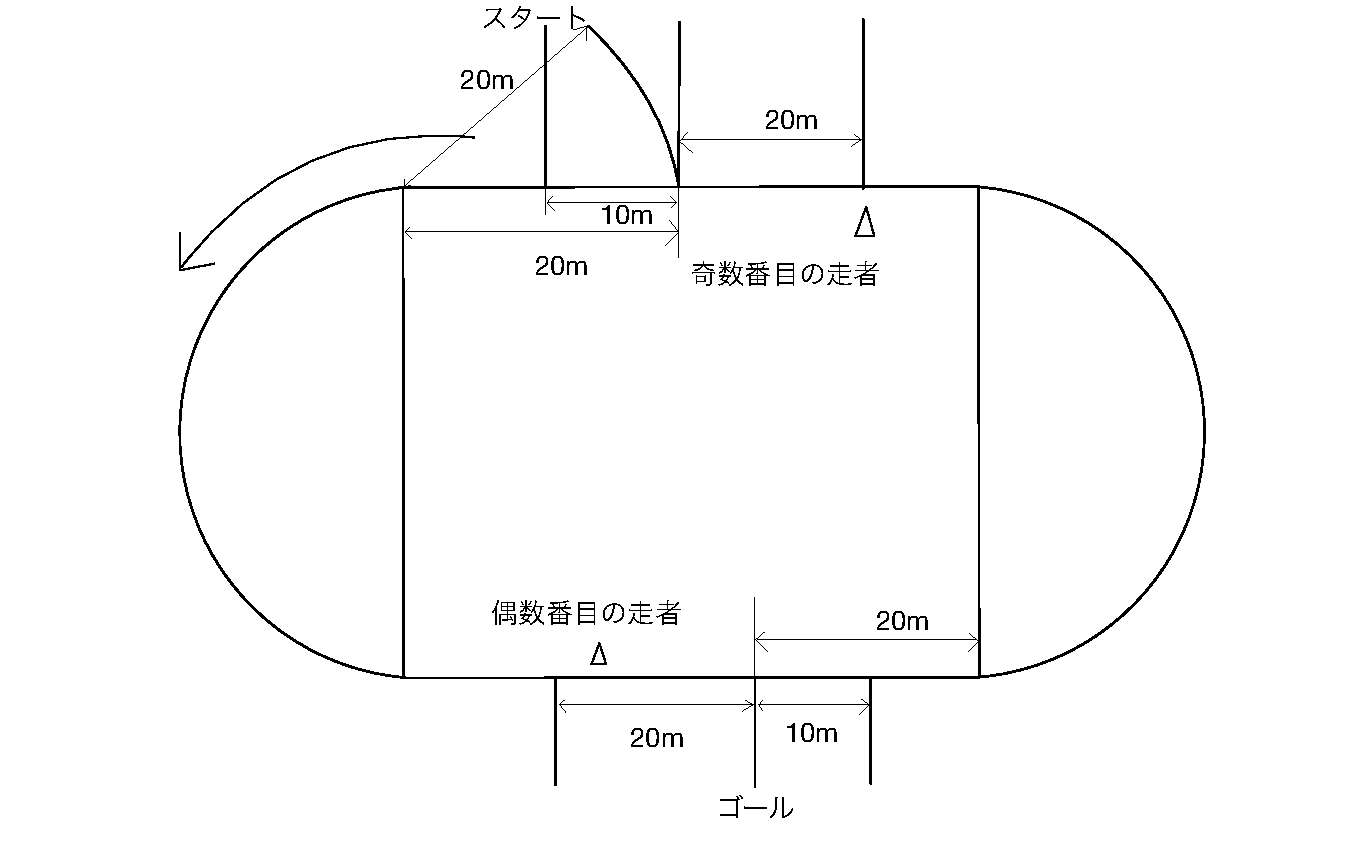
\includegraphics[width=12cm]{rire3.pdf}
    \caption{リレー競技図}
   \end{figure}
  \subsection{使用器具}
   \begin{table}[H]
    \begin{tabular}{cccc}
     物品名&数量&管理者&備考\\ \hline\hline
カラーコーン&10個&学生会体育委員会&高さ60cm\\
バトン&5個&学生会体育委員会&1個×5色\\
ゴールテープ&1個&学生会体育委員会&\\
ビブス&5枚&学生会体育委員会&1枚×5色\\
    \end{tabular}
   \end{table}
  \subsection{審判}
   学生会役員5人で行う。
   \begin{itemize}
    \item スタートの合図:1人
    \item バトンの受け渡し確認係:2人
    \item 選手の誘導確認係:2人
   \end{itemize}
  \subsection{その他の注意点}
   \begin{itemize}
    \item 各学科の5年生の体育委員はメンバー決めの際、5走者目に走ってもらう先生に事前に依頼し、メンバー表にはその先生の名前も記入し提出すること。
    \item 審判は走者の確認をしっかりと行う、特にアンカーが団長であることを確認すること。
   \end{itemize}
\clearpage
 \part*{各競技の配点}
  \begin{table}[H]
   \centering
   \begin{tabular}{l|ccccc}
    &1位&2位&3位&4位&5位\\ \hline\hline
    宅配競争&90&70&50&40&30\\
    借り人競争&130&80&60&50&40\\
    玉入れ&100&80&60&50&40\\
    リレー&150&100&80&60&50\\
   \end{tabular}
  \end{table}
{\large\bf 総合成績=競技得点×開閉会式の出席率の割合}\\
各学科の競技点数合計は昼休みに途中経過を発表し、閉会式に総合成績を発表する。

\section*{競技用ラインまとめ}
   \begin{figure}[H]
    \centering
    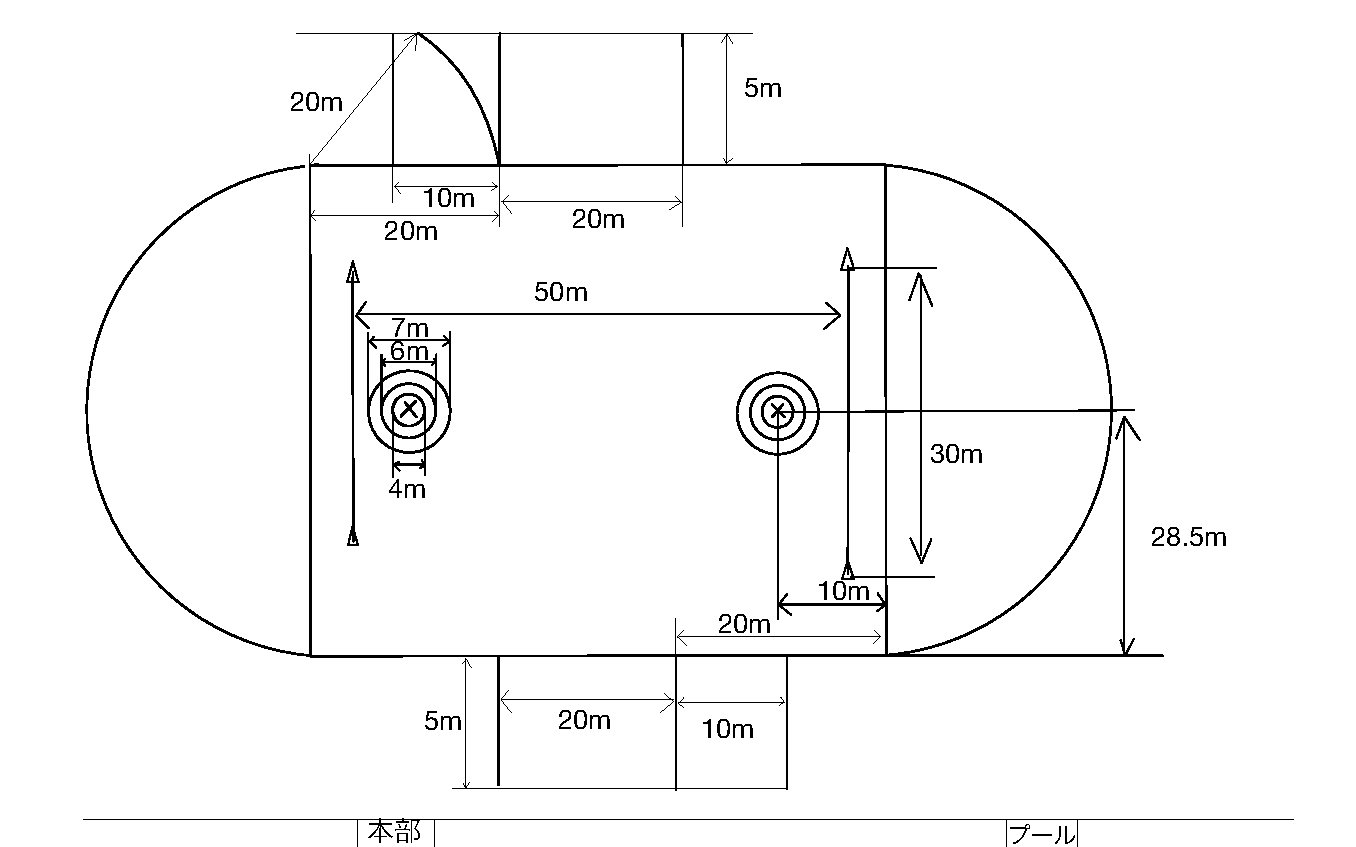
\includegraphics[width=12cm]{line.pdf}
    \caption{line}
   \end{figure}
 \clearpage
 \section{本部}
  \subsection{本部に必要な役員}
   通信長\&指揮×1、アナウンサー×2、得点係×2、人数確認係×5
  \subsection{本部に必要な物品}
\begin{table}[H]
\begin{tabular}{cccc}
     物品名&数量&管理者&備考\\ \hline\hline
 放送機材        & 一式  & 学生課              &  \\
 PC          & 1台  & 体育委員会  BGM再生用、表計算用 &  \\
 ホワイトボード     & 2個  & 総務部                &  \\
 ホワイトボードマーカー & 6本  & 総務部                &  \\
 本部用テント      & 2個  & 学生課            &  \\
 救急箱         & 1個  & 保健室              &  \\
 机           & 8個  & 学生課               &  \\
 椅子          & 15個 & 学生課   & 観客用も含む        \\
 学科プラカード     & 5個  & 体育委員会 &               \\
 単一電池        & 20個 & 体育委員会 & 放送機材用、予備4個    \\
 養生テープ       & 3個  & 総務部   &               \\
 トロフィー       & 1個  & 体育委員会 &               \\
 賞品          & 3個  & 体育委員会 &              
\end{tabular}
\end{table}
 \section{使用物品総覧}
\begin{table}[H]
\centering
\caption{使用物品}
\begin{tabular}{llll}
     物品名&数量&管理者&備考\\ \hline\hline
カラーコーン   & 12個  & 体育委員会 & 高さ60cm、予備2個 \\
紅玉       & 99個  & 体育委員会 & 予備9個        \\
白玉       & 99個  & 体育委員会 & 予備6個        \\
かご(紅白)   & 2個   & 体育委員会 & 最大4m44cm    \\
パン(競技用)  & 45個  & 体育委員会 & 100円、予備一個   \\
木材       & 3本   & 体育委員会 & 長さ2m        \\
賞品(パン食い) & 7セット & 体育委員会 & 部費7500円分    \\
紐        & 10本  & 体育委員会 & パン吊るす用      \\
バトン      & 5本   & 体育委員会 & 1本×5色       \\
ゴールテープ   & 1個   & 体育委員会 &             \\
ビブス      & 5枚   & 体育委員会 & 1枚×5色       \\
ダンボール    & 50箱分 & 体育委員会 & 300×300×150 \\
A4白紙     & 120枚 & 学生会   &             \\
マイク      & 1本   & 学生課   &            
\end{tabular}
\end{table}

\begin{table}[H]
\centering
\caption{共通物品}
\begin{tabular}{llll}
     物品名&数量&管理者&備考\\ \hline\hline
救急箱         & 1個    & 保健室   &                 \\
本部用テント      & 2個    & 学生課   &                 \\
長椅子         & 8個    & 学生課   &                 \\
パイプ椅子       & 15個   & 学生課   &            \\
トランシーバー     & 3個    & 学生課   &                 \\
放送機材        & 1式    & 学生課   &                 \\
ゴミ袋         & 10枚   & 学生課   &                 \\
台車          & 1台    & 学生課   &                 \\
ラインカー       & 4機    & 学生課   &                 \\
拡声器         &  5台   & 学生課   & 事前に確認したときは2つ       \\
消毒液         & 5個    & 学生課   & レース前の消毒用4個+予備1個 \\
ラインカー       & 1機    & 体育委員会 &                 \\
石灰          & 大2,小8 & 体育委員会 & 大20kg,小5kg      \\
メジャー        & 2個    & 体育委員会 &                 \\
ピストル        & 2丁    & 体育委員会 &                 \\
雷管          & 1箱    & 体育委員会 &                 \\
学科プラカード     & 5個    & 体育委員会 &                 \\
PC          & 1台    & 体育委員会 &                 \\
単一電池        & 20個   & 体育委員会 &                 \\
トロフィー       & 1個    & 体育委員会 &                 \\
賞品          & 3個    & 体育委員会 &                 \\
ホワイトボード     & 3個    & 総務部   &                 \\
ホワイトボードマーカー & 6本    & 総務部   & 黒赤各三本           \\
拡声器         & 2個    & 文化委員会 &                
\end{tabular}
\end{table}

\begin{table}[H]
\centering
\caption{購入物品}
\begin{tabular}{llll}
    物品名&数量&1つあたり&備考\\ \hline\hline
パン & 45個 & 100円 & 4500円  \\
賞品 & 3個  &      & 40000円
\end{tabular}
\end{table}
\clearpage
 \section{賞品}
総合成績が1位の学科にはトロフィーと賞品、2、3位の学科には賞品を閉会式に授与する。賞品の金額は1位から順に4000円×5学年の計20000円、2500円×5学年の計12500 円、1500円×5学年の計7500円とする。
 \section{雨天及び、コロナ等での中止について}
  \begin{itemize}
\item 体育祭決行または中止の判断は仮判断として前々日の天気と天気予報、最終決定として前日の昼休みの天気と天気予報から決める。
\item その判断は体育委員長・学生会長・学生主事で行う。
\item 10月12日が雨天だった場合、10月19日に延期する。
\item 10月19日が雨天だった場合クラスマッチは行わず中止する。
\item 緊急事態宣言、蔓延防止等充填措置、または特別警報が体育祭に重なった場合、中止を検討する。
\item 学生・教職員が感染した場合、中止を検討する。
\item 学生・教職員が濃厚接触者となった場合は実施を検討する。しかし、当該者は参加できない。
\item 臨時休業となった場合、感染・濃厚接触者に関わらず中止となる。
\end{itemize}
 \section{お問い合わせ}
意見・質問がある場合は本企画書表紙の総責任者の学内アドレスにメールするか、学生課を通して連絡をしてください。
\end{document}